%\begin{longtable}{|r l|p{2cm}|p{6cm}|p{2cm}|}
\begin{longtable}[H]{p{0.12\textwidth} p{0.2\textwidth} p{0.40\textwidth} p{0.17\textwidth}}\\
	\toprule
	\textbf{Requisito}	&	\textbf{Tipologia}	&	\textbf{Descrizione}	&	\textbf{Fonti}\\*
	\midrule
	\midrule

	\hypertarget{R-3V1}{R-3V1} & Vincolo Obbligatorio & La parte destinata ai creatori di domande e di questionari dovrà essere fruibile attraverso un PC & Capitolato \\*
	\midrule
	\hypertarget{R-3V2}{R-3V2} & Vincolo
	
	Obbligatorio & La parte server deve essere realizzata in Javascript con server node.js
	& Capitolato\\*
	\midrule
	\hypertarget{R-3V3}{R-3V3} & Vincolo
	
	Obbligatorio & La parte client dovrà essere eseguibile in un browser HTML5 & Capitolato\\*
	\midrule
	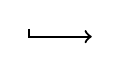
\begin{tikzpicture}
	\draw [->, thick] (0.2,0.2) -- (0.2,0.1) -- (1,0.1);
	\end{tikzpicture} \hypertarget{R-3V3.1}{R-3V3.1} & Vincolo
	
	Obbligatorio & L'applicazione funziona correttamente su Chrome versione 47.0.2526 e successive & Capitolato\\*
	\midrule
	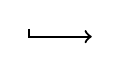
\begin{tikzpicture}
	\draw [->, thick] (0.2,0.2) -- (0.2,0.1) -- (1,0.1);
	\end{tikzpicture} \hypertarget{R-3V3.2}{R-3V3.2} & Vincolo
	
	Obbligatorio & L'applicazione funziona correttamente su Firefox versione 38.5.2esr e successive & Capitolato\\*
	\midrule
	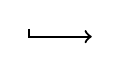
\begin{tikzpicture}
	\draw [->, thick] (0.2,0.2) -- (0.2,0.1) -- (1,0.1);
	\end{tikzpicture} \hypertarget{R-3V3.3}{R-3V3.3} & Vincolo
	
	Obbligatorio & L'applicazione funziona correttamente su Microsoft Edge versione 25.10586 e successive & Capitolato\\*
	\midrule
	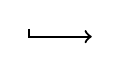
\begin{tikzpicture}
	\draw [->, thick] (0.2,0.2) -- (0.2,0.1) -- (1,0.1);
	\end{tikzpicture} \hypertarget{R-3V3.4}{R-3V3.4} & Vincolo
	
	Obbligatorio & L'applicazione funziona correttamente su Safari versione 9.0.2 e successive & Capitolato\\*
	\midrule
	\hypertarget{R-3V4}{R-3V4} & Vincolo
	
	Obbligatorio & L'applicazione deve utilizzare fogli stile CSS3 per l’ aspetto estetico & Capitolato\\*
	\midrule
	\hypertarget{R-3V5}{R-3V5} & Vincolo
	
	Obbligatorio & L'applicazione deve utilizzare Javascript per la parte attiva del client & Capitolato\\*
	\midrule
	\hypertarget{R-3V6}{R-3V6} & Vincolo
	
	Obbligatorio & La parte destinata agli esaminandi dovrà funzionare con qualunque dispositivo: dal Personal Computer, ai Tablet ed agli SmartPhone attraverso browser & Capitolato\\*
	\midrule
	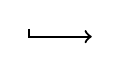
\begin{tikzpicture}
	\draw [->, thick] (0.2,0.2) -- (0.2,0.1) -- (1,0.1);
	\end{tikzpicture} \hypertarget{R-3V6.1}{R-3V6.1} & Vincolo
	
	Obbligatorio & La parte destinata agli esaminandi dovrà funzionare si smartphone e tablet iOS dalla versione iOS6 & Capitolato\\*
	\midrule
	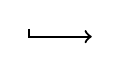
\begin{tikzpicture}
	\draw [->, thick] (0.2,0.2) -- (0.2,0.1) -- (1,0.1);
	\end{tikzpicture} \hypertarget{R-3V6.2}{R-3V6.2} & Vincolo
	
	Obbligatorio & La parte destinata agli esaminandi dovrà funzionare su Android dalla versione 4.0 & Capitolato\\*
	\midrule
	\hypertarget{R-3F7}{R-3F7} & Funzionale
	
	Obbligatorio & Il sistema deve gestire questionari & Capitolato
	
	\hyperlink{UC19}{UC19}\\*
	\midrule
	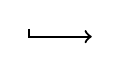
\begin{tikzpicture}
	\draw [->, thick] (0.2,0.2) -- (0.2,0.1) -- (1,0.1);
	\end{tikzpicture} \hypertarget{R-3F7.1}{R-3F7.1} & Funzionale
	
	Obbligatorio & L'applicazione deve archiviare questionari in un server, suddivisi per argomento
	& Capitolato\\*
	\midrule
	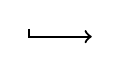
\begin{tikzpicture}
	\draw [->, thick] (0.2,0.2) -- (0.2,0.1) -- (1,0.1);
	\end{tikzpicture} \hypertarget{R-3F7.2}{R-3F7.2} & Funzionale
	
	Obbligatorio & L'applicazione deve tradurre da QML a HTML le domande archiviate & Capitolato
	
	\hyperlink{UC18.10}{UC18.10}
	
	\hyperlink{UC18}{UC18}
	
	\hyperlink{UC19}{UC19}
	
	\hyperlink{UC6.1}{UC6.1}\\*
	\midrule
	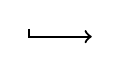
\begin{tikzpicture}
	\draw [->, thick] (0.2,0.2) -- (0.2,0.1) -- (1,0.1);
	\end{tikzpicture} \hypertarget{R-3F7.3}{R-3F7.3} & Funzionale
	
	Obbligatorio & L'applicazione deve proporre questionari preconfezionati & Capitolato
	
	\hyperlink{UC19}{UC19}\\*
	\midrule
	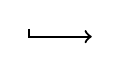
\begin{tikzpicture}
	\draw [->, thick] (0.2,0.2) -- (0.2,0.1) -- (1,0.1);
	\end{tikzpicture} \hypertarget{R-3F7.4}{R-3F7.4} & Funzionale
	
	Obbligatorio & L'applicazione deve valutare le risposte fornite dall'utente & Capitolato
	
	\hyperlink{UC6.11}{UC6.11}
	
	\hyperlink{UC6}{UC6}
	
	\hyperlink{UC8}{UC8}\\*
	\midrule
	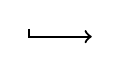
\begin{tikzpicture}
	\draw [->, thick] (0.2,0.2) -- (0.2,0.1) -- (1,0.1);
	\end{tikzpicture} \hypertarget{R-3F7.5}{R-3F7.5} & Funzionale
	
	Obbligatorio & Le domande dovranno essere raccolte attraverso uno specifico linguaggio, che chiameremo Quiz Markup Language (QML), studiato per descrivere quiz
	& Capitolato
	
	\hyperlink{UC18.1.2}{UC18.1.2}\\*
	\midrule
	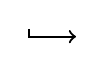
\begin{tikzpicture}
	\draw [->, thick] (0.4,0.2) -- (0.4,0.1) -- (1,0.1);
	\end{tikzpicture} \hypertarget{R-3F7.5.1}{R-3F7.5.1} & Funzionale
	
	Obbligatorio & Il QML deve essere un linguaggio semplice con un parsing ad hoc definito dal gruppo. La sintassi per scrivere il testo della domanda deve essere unica, la sintassi per le risposte è dipendente dal tipo di domanda & Capitolato
	
	\hyperlink{UC18.1.2}{UC18.1.2}\\*
	\midrule
	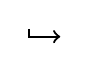
\begin{tikzpicture}
	\draw [->, thick] (0.6,0.2) -- (0.6,0.1) -- (1,0.1);
	\end{tikzpicture} \hypertarget{R-2F7.5.1.1}{R-2F7.5.1.1} & Funzionale
	
	Opzionale & Il QML deve permettere l'inserimento di testo in grassetto & \hyperlink{UC18.1.2}{UC18.1.2}\\*
	\midrule
	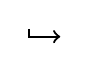
\begin{tikzpicture}
	\draw [->, thick] (0.6,0.2) -- (0.6,0.1) -- (1,0.1);
	\end{tikzpicture} \hypertarget{R-3F7.5.1.2}{R-3F7.5.1.2} & Funzionale
	
	Obbligatorio & Il QML deve permettere l'inserimento di immagini & Capitolato
	
	\hyperlink{UC18.1.2}{UC18.1.2}\\*
	\midrule
	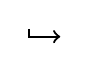
\begin{tikzpicture}
	\draw [->, thick] (0.6,0.2) -- (0.6,0.1) -- (1,0.1);
	\end{tikzpicture} \hypertarget{R-2F7.5.1.3}{R-2F7.5.1.3} & Funzionale
	
	Opzionale & Il QML deve permettere l'inserimento di testo in corsivo & \hyperlink{UC18.1.2}{UC18.1.2}\\*
	\midrule
	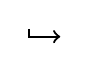
\begin{tikzpicture}
	\draw [->, thick] (0.6,0.2) -- (0.6,0.1) -- (1,0.1);
	\end{tikzpicture} \hypertarget{R-2F7.5.1.4}{R-2F7.5.1.4} & Funzionale
	
	Opzionale & Il QML deve permettere l'inserimento di tabelle & \hyperlink{UC18.1.2}{UC18.1.2}\\*
	\midrule
	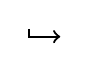
\begin{tikzpicture}
	\draw [->, thick] (0.6,0.2) -- (0.6,0.1) -- (1,0.1);
	\end{tikzpicture} \hypertarget{R-2F7.5.1.5}{R-2F7.5.1.5} & Funzionale
	
	Opzionale & Il QML deve permettere di definire un punteggio per ogni risposta & \hyperlink{UC18.1.2}{UC18.1.2}\\*
	\midrule
	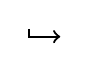
\begin{tikzpicture}
	\draw [->, thick] (0.6,0.2) -- (0.6,0.1) -- (1,0.1);
	\end{tikzpicture} \hypertarget{R-3F7.5.1.6}{R-3F7.5.1.6} & Funzionale
	
	Obbligatorio & Il QML deve permettere di definire il tipo di domanda & \hyperlink{UC18.1.2}{UC18.1.2}\\*
	\midrule
	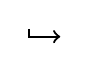
\begin{tikzpicture}
	\draw [->, thick] (0.6,0.2) -- (0.6,0.1) -- (1,0.1);
	\end{tikzpicture} \hypertarget{R-2F7.5.1.7}{R-2F7.5.1.7} & Funzionale
	
	Opzionale & Il QML deve permettere l'inserimento di video & \hyperlink{UC18.1.2}{UC18.1.2}
	
	\hyperlink{UC18.1.5}{UC18.1.5}\\*
	\midrule
	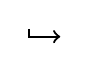
\begin{tikzpicture}
	\draw [->, thick] (0.6,0.2) -- (0.6,0.1) -- (1,0.1);
	\end{tikzpicture} \hypertarget{R-2F7.5.1.8}{R-2F7.5.1.8} & Funzionale
	
	Opzionale & Il QML deve permettere l'inserimento di audio & \hyperlink{UC18.1.2}{UC18.1.2}
	
	\hyperlink{UC18.1.5}{UC18.1.5}\\*
	\midrule
	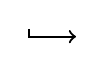
\begin{tikzpicture}
	\draw [->, thick] (0.4,0.2) -- (0.4,0.1) -- (1,0.1);
	\end{tikzpicture} \hypertarget{R-2F7.5.2}{R-2F7.5.2} & Funzionale
	
	Opzionale & Il QML può gestire risposte a scelta multipla, a riempimento di parole omesse, ad associazione, a risposta aperta, con testi e immagini & Capitolato
	
	\hyperlink{UC18.1}{UC18.1}
	
	\hyperlink{UC18.5}{UC18.5}
	
	\hyperlink{UC18.7}{UC18.7}
	
	\hyperlink{UC18.8}{UC18.8}
	
	\hyperlink{UC18.9}{UC18.9}\\*
	\midrule
	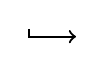
\begin{tikzpicture}
	\draw [->, thick] (0.4,0.2) -- (0.4,0.1) -- (1,0.1);
	\end{tikzpicture} \hypertarget{R-3F7.5.3}{R-3F7.5.3} & Funzionale
	
	Obbligatorio & Le domande scritte in QML devono essere editabili dall'utente & Proponente
	
	\hyperlink{UC18.1}{UC18.1}\\*
	\midrule
	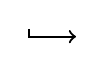
\begin{tikzpicture}
	\draw [->, thick] (0.4,0.2) -- (0.4,0.1) -- (1,0.1);
	\end{tikzpicture} \hypertarget{R-2F7.5.4}{R-2F7.5.4} & Funzionale
	
	Opzionale & Le domande possono essere inserite e editabili attraverso interfaccia grafica & Proponente
	
	\hyperlink{UC18.1.5}{UC18.1.5}\\*
	\midrule
	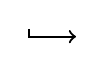
\begin{tikzpicture}
	\draw [->, thick] (0.4,0.2) -- (0.4,0.1) -- (1,0.1);
	\end{tikzpicture} \hypertarget{R-3F7.5.5}{R-3F7.5.5} & Funzionale
	
	Obbligatorio & Il QML deve gestire risposte vero/falso e risposte a scelta multipla con testi e immagini & Capitolato
	
	\hyperlink{UC18.1}{UC18.1}
	
	\hyperlink{UC18.4}{UC18.4}
	
	\hyperlink{UC18.6}{UC18.6}\\*
	\midrule
	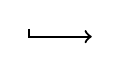
\begin{tikzpicture}
	\draw [->, thick] (0.2,0.2) -- (0.2,0.1) -- (1,0.1);
	\end{tikzpicture} \hypertarget{R-2F7.6}{R-2F7.6} & Funzionale
	
	Opzionale & Il sistema deve gestire sia questionari pubblici che privati attraverso la creazione di classi la cui iscrizione è protetta da password & Proponente
	
	\hyperlink{UC20.1}{UC20.1}
	
	\hyperlink{UC7}{UC7}\\*
	\midrule
	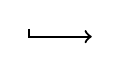
\begin{tikzpicture}
	\draw [->, thick] (0.2,0.2) -- (0.2,0.1) -- (1,0.1);
	\end{tikzpicture} \hypertarget{R-3F7.7}{R-3F7.7} & Funzionale
	
	Obbligatorio & I docenti costruiranno questionari scegliendo tra le domande archiviate nel server & Capitolato
	
	\hyperlink{UC19.1}{UC19.1}
	
	\hyperlink{UC19}{UC19}\\*
	\midrule
	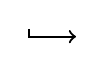
\begin{tikzpicture}
	\draw [->, thick] (0.4,0.2) -- (0.4,0.1) -- (1,0.1);
	\end{tikzpicture} \hypertarget{R-3F7.7.1}{R-3F7.7.1} & Funzionale
	
	Obbligatorio & Il sistema deve segnalare un errore nel caso un questionario creato non contenga domande & \hyperlink{UC19.1}{UC19.1}
	
	\hyperlink{UC19.4}{UC19.4}
	
	\hyperlink{UC19}{UC19}\\*
	\midrule
	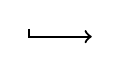
\begin{tikzpicture}
	\draw [->, thick] (0.2,0.2) -- (0.2,0.1) -- (1,0.1);
	\end{tikzpicture} \hypertarget{R-2F7.8}{R-2F7.8} & Funzionale
	
	Opzionale & Il sistema deve offrire la possibilità di creare dinamicamente i questionari & Capitolato\\*
	\midrule
	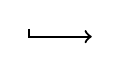
\begin{tikzpicture}
	\draw [->, thick] (0.2,0.2) -- (0.2,0.1) -- (1,0.1);
	\end{tikzpicture} \hypertarget{R-2F7.9}{R-2F7.9} & Funzionale
	
	Opzionale & L'applicazione deve essere predisposta ad un sistema di feedback per i questionari & Capitolato
	
	\hyperlink{UC6.10}{UC6.10}\\*
	\midrule
	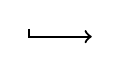
\begin{tikzpicture}
	\draw [->, thick] (0.2,0.2) -- (0.2,0.1) -- (1,0.1);
	\end{tikzpicture} \hypertarget{R-2F7.10}{R-2F7.10} & Funzionale
	
	Opzionale & Il sistema deve permettere la raccolta dei dati relativi a questionari svolti & Capitolato
	
	\hyperlink{UC8}{UC8}\\*
	\midrule
	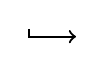
\begin{tikzpicture}
	\draw [->, thick] (0.4,0.2) -- (0.4,0.1) -- (1,0.1);
	\end{tikzpicture} \hypertarget{R-2F7.10.1}{R-2F7.10.1} & Funzionale
	
	Opzionale & Il sistema deve permettere la rivisitazione del test svolto e dei risultati ottenuti & Capitolato
	
	\hyperlink{UC8}{UC8}\\*
	\midrule
	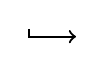
\begin{tikzpicture}
	\draw [->, thick] (0.4,0.2) -- (0.4,0.1) -- (1,0.1);
	\end{tikzpicture} \hypertarget{R-2F7.10.2}{R-2F7.10.2} & Funzionale
	
	Opzionale & Il sistema deve offrire la possibilità di analizzare i dati raccolti dai test effettuati & Capitolato
	
	\hyperlink{UC8.2}{UC8.2}
	
	\hyperlink{UC8}{UC8}\\*
	\midrule
	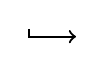
\begin{tikzpicture}
	\draw [->, thick] (0.4,0.2) -- (0.4,0.1) -- (1,0.1);
	\end{tikzpicture} \hypertarget{R-2F7.10.3}{R-2F7.10.3} & Funzionale
	
	Opzionale & Il sistema deve offrire la possibilità di visualizzazione sotto forma di grafico delle statistiche dei dati raccolti & Capitolato
	
	\hyperlink{UC8.3}{UC8.3}
	
	\hyperlink{UC8}{UC8}\\*
	\midrule
	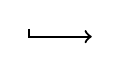
\begin{tikzpicture}
	\draw [->, thick] (0.2,0.2) -- (0.2,0.1) -- (1,0.1);
	\end{tikzpicture} \hypertarget{R-3F7.11}{R-3F7.11} & Funzionale
	
	Obbligatorio & Il sistema deve prevedere la gestione di domande & \hyperlink{UC18}{UC18}
	
	\hyperlink{UC19.1.1}{UC19.1.1}
	
	\hyperlink{UC19.1.2}{UC19.1.2}
	
	\hyperlink{UC19}{UC19}\\*
	\midrule
	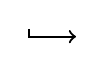
\begin{tikzpicture}
	\draw [->, thick] (0.4,0.2) -- (0.4,0.1) -- (1,0.1);
	\end{tikzpicture} \hypertarget{R-3F7.11.1}{R-3F7.11.1} & Funzionale
	
	Obbligatorio & Il sistema deve consentire ad un docente di inserire una nuova domanda & \hyperlink{UC18.1}{UC18.1}
	
	\hyperlink{UC18}{UC18}\\*
	\midrule
	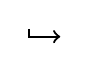
\begin{tikzpicture}
	\draw [->, thick] (0.6,0.2) -- (0.6,0.1) -- (1,0.1);
	\end{tikzpicture} \hypertarget{R-3F7.11.1.1}{R-3F7.11.1.1} & Funzionale
	
	Obbligatorio & Un docente deve poter selezionare gli argomenti di una domanda & \hyperlink{UC18.1.1}{UC18.1.1}
	
	\hyperlink{UC18.1}{UC18.1}
	
	\hyperlink{UC18}{UC18}\\*
	\midrule
	\begin{tikzpicture}
	\draw [->, thick] (0.8,0.2) -- (0.8,0.1) -- (1,0.1);
	\end{tikzpicture} \hypertarget{R-3F7.11.1.1.1}{R-3F7.11.1.1.1} & Funzionale
	
	Obbligatorio & Il sistema deve segnalare un errore nel caso non venga selezionato alcun argomento per una nuova domanda & \hyperlink{UC18.1.1}{UC18.1.1}
	
	\hyperlink{UC18.1.4}{UC18.1.4}
	
	\hyperlink{UC18}{UC18}
	
	\hyperlink{UC19.1.1}{UC19.1.1}\\*
	\midrule
	\begin{tikzpicture}
	\draw [->, thick] (0.8,0.2) -- (0.8,0.1) -- (1,0.1);
	\end{tikzpicture} \hypertarget{R-3F7.11.1.1.2}{R-3F7.11.1.1.2} & Funzionale
	
	Obbligatorio & Il sistema deve segnalare un errore nel caso ci siano argomenti associati ad una domanda modificata & \hyperlink{UC18.2.5}{UC18.2.5}\\*
	\midrule
	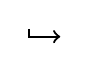
\begin{tikzpicture}
	\draw [->, thick] (0.6,0.2) -- (0.6,0.1) -- (1,0.1);
	\end{tikzpicture} \hypertarget{R-3F7.11.1.2}{R-3F7.11.1.2} & Funzionale
	
	Obbligatorio & Un docente deve comporre la domanda da inserire in QML & \hyperlink{UC18.1.2}{UC18.1.2}
	
	\hyperlink{UC18}{UC18}
	
	\hyperlink{UC19.1.1}{UC19.1.1}\\*
	\midrule
	\begin{tikzpicture}
	\draw [->, thick] (0.8,0.2) -- (0.8,0.1) -- (1,0.1);
	\end{tikzpicture} \hypertarget{R-3F7.11.1.2.1}{R-3F7.11.1.2.1} & Funzionale
	
	Obbligatorio & Il sistema deve segnalare un errore nel caso di inserimento QML non valido & \hyperlink{UC18.1.2}{UC18.1.2}
	
	\hyperlink{UC18.1.3}{UC18.1.3}
	
	\hyperlink{UC18.2.4}{UC18.2.4}
	
	\hyperlink{UC18}{UC18}
	
	\hyperlink{UC19.1.1}{UC19.1.1}\\*
	\midrule
	\begin{tikzpicture}
	\draw [->, thick] (0.8,0.2) -- (0.8,0.1) -- (1,0.1);
	\end{tikzpicture} \hypertarget{R-3F7.11.1.2.2}{R-3F7.11.1.2.2} & Funzionale
	
	Obbligatorio & Il docente deve poter inserire domande di tipo vero/falso & \hyperlink{UC18.1}{UC18.1}
	
	\hyperlink{UC18.4}{UC18.4}\\*
	\midrule
	\begin{tikzpicture}
	\draw [->, thick] (0.8,0.2) -- (0.8,0.1) -- (1,0.1);
	\end{tikzpicture} \hypertarget{R-3F7.11.1.2.3}{R-3F7.11.1.2.3} & Funzionale
	
	Obbligatorio & Il docente deve poter inserire domande a scelta multipla & \hyperlink{UC18.1}{UC18.1}
	
	\hyperlink{UC18.5}{UC18.5}\\*
	\midrule
	\begin{tikzpicture}
	\draw [->, thick] (0.8,0.2) -- (0.8,0.1) -- (1,0.1);
	\end{tikzpicture} \hypertarget{R-1F7.11.1.2.4}{R-1F7.11.1.2.4} & Funzionale
	
	Desiderabile & Il docente deve poter inserire domande a risposta multipla & \hyperlink{UC18.1}{UC18.1}
	
	\hyperlink{UC18.6}{UC18.6}\\*
	\midrule
	\begin{tikzpicture}
	\draw [->, thick] (0.8,0.2) -- (0.8,0.1) -- (1,0.1);
	\end{tikzpicture} \hypertarget{R-1F7.11.1.2.5}{R-1F7.11.1.2.5} & Funzionale
	
	Desiderabile & Il docente deve poter inserire domande di tipo testo con parole omesse & \hyperlink{UC18.1}{UC18.1}
	
	\hyperlink{UC18.7}{UC18.7}\\*
	\midrule
	\begin{tikzpicture}
	\draw [->, thick] (0.8,0.2) -- (0.8,0.1) -- (1,0.1);
	\end{tikzpicture} \hypertarget{R-1F7.11.1.2.6}{R-1F7.11.1.2.6} & Funzionale
	
	Desiderabile & Il docente deve poter inserire domande con associazione di parole & \hyperlink{UC18.1}{UC18.1}
	
	\hyperlink{UC18.8}{UC18.8}\\*
	\midrule
	\begin{tikzpicture}
	\draw [->, thick] (0.8,0.2) -- (0.8,0.1) -- (1,0.1);
	\end{tikzpicture} \hypertarget{R-2F7.11.1.2.7}{R-2F7.11.1.2.7} & Funzionale
	
	Opzionale & Il docente deve poter inserire domande a risposta aperta & \hyperlink{UC18.1}{UC18.1}
	
	\hyperlink{UC18.9}{UC18.9}\\*
	\midrule
	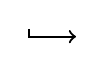
\begin{tikzpicture}
	\draw [->, thick] (0.4,0.2) -- (0.4,0.1) -- (1,0.1);
	\end{tikzpicture} \hypertarget{R-3F7.11.2}{R-3F7.11.2} & Funzionale
	
	Obbligatorio & Il sistema deve consentire ad un docente di modificare una domanda & \hyperlink{UC18.2.1}{UC18.2.1}
	
	\hyperlink{UC18.2.2}{UC18.2.2}
	
	\hyperlink{UC18.2.3}{UC18.2.3}
	
	\hyperlink{UC18.2}{UC18.2}
	
	\hyperlink{UC18}{UC18}\\*
	\midrule
	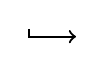
\begin{tikzpicture}
	\draw [->, thick] (0.4,0.2) -- (0.4,0.1) -- (1,0.1);
	\end{tikzpicture} \hypertarget{R-3F7.11.3}{R-3F7.11.3} & Funzionale
	
	Obbligatorio & Il sistema deve consentire ad un docente di eliminare una propria domanda presente nel sistema & \hyperlink{UC18.3}{UC18.3}
	
	\hyperlink{UC18}{UC18}\\*
	\midrule
	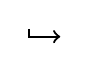
\begin{tikzpicture}
	\draw [->, thick] (0.6,0.2) -- (0.6,0.1) -- (1,0.1);
	\end{tikzpicture} \hypertarget{R-3F7.11.3.1}{R-3F7.11.3.1} & Funzionale
	
	Obbligatorio & Il sistema deve permettere la visualizzazione di un messaggio di errore se il docente tenta di cancellare una propria domanda che è presente in questionari & \hyperlink{UC18.11}{UC18.11}\\*
	\midrule
	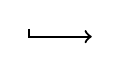
\begin{tikzpicture}
	\draw [->, thick] (0.2,0.2) -- (0.2,0.1) -- (1,0.1);
	\end{tikzpicture} \hypertarget{R-3F7.12}{R-3F7.12} & Funzionale
	
	Obbligatorio & il sistema deve dare la possibilità al docente di modificare il proprio questionario & \hyperlink{UC19.2}{UC19.2}
	
	\hyperlink{UC19}{UC19}\\*
	\midrule
	\begin{tikzpicture}
	\draw [->, thick] (0.4,0.2) -- (0.4,0.1) -- (1,0.1);
	\end{tikzpicture} \hypertarget{R-3F7.12.1}{R-3F7.12.1} & Funzionale
	
	Obbligatorio & Il sistema deve dare la possibilità di ricercare un questionario & \hyperlink{UC9}{UC9}\\*
	\midrule
	\begin{tikzpicture}
	\draw [->, thick] (0.4,0.2) -- (0.4,0.1) -- (1,0.1);
	\end{tikzpicture} \hypertarget{R-3F7.12.2}{R-3F7.12.2} & Funzionale
	
	Obbligatorio & Il sistema deve dare la possibile al docente di aggiungere al questionario già fatto una domanda. & \hyperlink{UC19.2.1}{UC19.2.1}
	
	\hyperlink{UC19}{UC19}\\*
	\midrule
	\begin{tikzpicture}
	\draw [->, thick] (0.4,0.2) -- (0.4,0.1) -- (1,0.1);
	\end{tikzpicture} \hypertarget{R-3F7.12.3}{R-3F7.12.3} & Funzionale
	
	Obbligatorio & Il sistema deve dare la possibilità al docente di togliere domande precedentemente aggiunte al questionario & \hyperlink{UC19.2.2}{UC19.2.2}
	
	\hyperlink{UC19}{UC19}\\*
	\midrule
	\begin{tikzpicture}
	\draw [->, thick] (0.4,0.2) -- (0.4,0.1) -- (1,0.1);
	\end{tikzpicture} \hypertarget{R-3F7.12.4}{R-3F7.12.4} & Funzionale
	
	Obbligatorio & Il sistema deve consentire ad un docente di modificare gli argomenti di un proprio questionario & \hyperlink{UC19.2.3}{UC19.2.3}
	
	\hyperlink{UC19.2}{UC19.2}
	
	\hyperlink{UC19}{UC19}\\*
	\midrule
	\begin{tikzpicture}
	\draw [->, thick] (0.2,0.2) -- (0.2,0.1) -- (1,0.1);
	\end{tikzpicture} \hypertarget{R-3F7.13}{R-3F7.13} & Funzionale
	
	Obbligatorio & Il sistema deve dare la possibilità al docente di eliminare il proprio questionario & \hyperlink{UC19.3}{UC19.3}
	
	\hyperlink{UC19}{UC19}\\*
	\midrule
	\begin{tikzpicture}
	\draw [->, thick] (0.2,0.2) -- (0.2,0.1) -- (1,0.1);
	\end{tikzpicture} \hypertarget{R-3F7.14}{R-3F7.14} & Funzionale
	
	Obbligatorio & Il sistema deve dare la possibilità al docente di inserire un nuovo questionario & \hyperlink{UC19.1}{UC19.1}\\*
	\midrule
	\begin{tikzpicture}
	\draw [->, thick] (0.4,0.2) -- (0.4,0.1) -- (1,0.1);
	\end{tikzpicture} \hypertarget{R-3F7.14.1}{R-3F7.14.1} & Funzionale
	
	Obbligatorio & Un docente deve poter specificare gli argomenti di un nuovo questionario & \hyperlink{UC19.1.3}{UC19.1.3}\\*
	\midrule
	\hypertarget{R-3F8}{R-3F8} & Funzionale
	
	Obbligatorio & Il sistema deve avere almeno 3 tipi di utenti: amministratore, docente e studente & Capitolato\\*
	\midrule
	\hypertarget{R-3F9}{R-3F9} & Funzionale
	
	Obbligatorio & Il sistema deve gestire la registrazione di un utente & \hyperlink{UC2}{UC2}\\*
	\midrule
	\begin{tikzpicture}
	\draw [->, thick] (0.2,0.2) -- (0.2,0.1) -- (1,0.1);
	\end{tikzpicture} \hypertarget{R-3F9.1}{R-3F9.1} & Funzionale
	
	Obbligatorio & Il sistema deve già possedere un proprietario all'installazione del sistema & Interno\\*
	\midrule
	\begin{tikzpicture}
	\draw [->, thick] (0.2,0.2) -- (0.2,0.1) -- (1,0.1);
	\end{tikzpicture} \hypertarget{R-3F9.2}{R-3F9.2} & Funzionale
	
	Obbligatorio & La registrazione di un utente richiede l’inserimento di uno username, password e nome completo  & \hyperlink{UC2.1}{UC2.1}
	
	\hyperlink{UC2.2}{UC2.2}
	
	\hyperlink{UC2.3}{UC2.3}\\*
	\midrule
	\begin{tikzpicture}
	\draw [->, thick] (0.4,0.2) -- (0.4,0.1) -- (1,0.1);
	\end{tikzpicture} \hypertarget{R-3F9.2.1}{R-3F9.2.1} & Funzionale
	
	Obbligatorio & Il sistema deve segnalare un errore nel caso non vengano inseriti tutti i campi necessari per la registrazione & \hyperlink{UC2.4}{UC2.4}
	
	\hyperlink{UC2.5}{UC2.5}
	
	\hyperlink{UC2.6}{UC2.6}
	
	\hyperlink{UC2.7}{UC2.7}\\*
	\midrule
	\begin{tikzpicture}
	\draw [->, thick] (0.4,0.2) -- (0.4,0.1) -- (1,0.1);
	\end{tikzpicture} \hypertarget{R-3F9.2.2}{R-3F9.2.2} & Funzionale
	
	Obbligatorio & La registrazione di uno utente deve richiedere l'inserimento delle informazioni personali & \hyperlink{UC2.1}{UC2.1}\\*
	\midrule
	\begin{tikzpicture}
	\draw [->, thick] (0.2,0.2) -- (0.2,0.1) -- (1,0.1);
	\end{tikzpicture} \hypertarget{R-3F9.3}{R-3F9.3} & Funzionale
	
	Obbligatorio & Il sistema deve permettere la visualizzazione di un messaggio di errore se l'username dell' utente è già presente nel sistema & \hyperlink{UC2.7}{UC2.7}\\*
	\midrule
	\begin{tikzpicture}
	\draw [->, thick] (0.2,0.2) -- (0.2,0.1) -- (1,0.1);
	\end{tikzpicture} \hypertarget{R-3F9.4}{R-3F9.4} & Funzionale
	
	Obbligatorio & Il sistema deve permettere la visualizzazione di un messaggio di errore se la password dell'utente è troppo corta & \hyperlink{UC2.6}{UC2.6}\\*
	\midrule
	\begin{tikzpicture}
	\draw [->, thick] (0.2,0.2) -- (0.2,0.1) -- (1,0.1);
	\end{tikzpicture} \hypertarget{R-3F9.5}{R-3F9.5} & Funzionale
	
	Obbligatorio & Il sistema deve segnalare un errore se viene inserito un username già utilizzato & \hyperlink{UC2.7}{UC2.7}\\*
	\midrule
	\hypertarget{R-3V10}{R-3V10} & Vincolo
	
	Obbligatorio & Il database server side deve essere MongoDB & Capitolato
	
	Interno\\*
	\midrule
	\hypertarget{R-3F11}{R-3F11} & Funzionale
	
	Obbligatorio & Il sistema deve gestire le azioni di amministratore & \hyperlink{UC31}{UC31}\\*
	\midrule
	\begin{tikzpicture}
	\draw [->, thick] (0.2,0.2) -- (0.2,0.1) -- (1,0.1);
	\end{tikzpicture} \hypertarget{R-3F11.1}{R-3F11.1} & Funzionale
	
	Obbligatorio & L'amministratore deve poter cambiare il ruolo di un utente con grado inferiore al proprio in un ruolo con grado inferiore al proprio & \hyperlink{UC31.1}{UC31.1}
	
	\hyperlink{UC31}{UC31}\\*
	\midrule
	\begin{tikzpicture}
	\draw [->, thick] (0.2,0.2) -- (0.2,0.1) -- (1,0.1);
	\end{tikzpicture} \hypertarget{R-3F11.2}{R-3F11.2} & Funzionale
	
	Obbligatorio & Il sistema deve dare la possibilità ad un amministratore di eliminare un utente di ruolo inferiore al proprio & \hyperlink{UC31.2}{UC31.2}
	
	\hyperlink{UC31}{UC31}\\*
	\midrule
	\hypertarget{R-2F12}{R-2F12} & Funzionale
	
	Opzionale & Il sistema deve prevedere la gestione di classi da parte di un docente & \hyperlink{UC20}{UC20}\\*
	\midrule
	\begin{tikzpicture}
	\draw [->, thick] (0.2,0.2) -- (0.2,0.1) -- (1,0.1);
	\end{tikzpicture} \hypertarget{R-2F12.1}{R-2F12.1} & Funzionale
	
	Opzionale & Un docente deve avere la possibilità di creare una nuova classe & \hyperlink{UC20.1}{UC20.1}
	
	\hyperlink{UC20}{UC20}\\*
	\midrule
	\begin{tikzpicture}
	\draw [->, thick] (0.4,0.2) -- (0.4,0.1) -- (1,0.1);
	\end{tikzpicture} \hypertarget{R-2F12.1.1}{R-2F12.1.1} & Funzionale
	
	Opzionale & Un docente deve poter specificare il nome della nuova classe & \hyperlink{UC20.1.1}{UC20.1.1}
	
	\hyperlink{UC20.1}{UC20.1}
	
	\hyperlink{UC20}{UC20}\\*
	\midrule
	\begin{tikzpicture}
	\draw [->, thick] (0.6,0.2) -- (0.6,0.1) -- (1,0.1);
	\end{tikzpicture} \hypertarget{R-2F12.1.1.1}{R-2F12.1.1.1} & Funzionale
	
	Opzionale & Nel caso il nome della classe sia già presente il sistema deve segnalare un errore & \hyperlink{UC20.1.1}{UC20.1.1}
	
	\hyperlink{UC20.1}{UC20.1}
	
	\hyperlink{UC20.4}{UC20.4}
	
	\hyperlink{UC20}{UC20}\\*
	\midrule
	\begin{tikzpicture}
	\draw [->, thick] (0.4,0.2) -- (0.4,0.1) -- (1,0.1);
	\end{tikzpicture} \hypertarget{R-2F12.1.2}{R-2F12.1.2} & Funzionale
	
	Opzionale & Un docente deve poter specificare gli argomenti di una nuova classe & \hyperlink{UC20.1.2}{UC20.1.2}
	
	\hyperlink{UC20.1}{UC20.1}
	
	\hyperlink{UC20}{UC20}\\*
	\midrule
	\begin{tikzpicture}
	\draw [->, thick] (0.4,0.2) -- (0.4,0.1) -- (1,0.1);
	\end{tikzpicture} \hypertarget{R-2F12.1.3}{R-2F12.1.3} & Funzionale
	
	Opzionale & Un docente deve poter specificare la password relativa ad una nuova classe & \hyperlink{UC20.1.3}{UC20.1.3}
	
	\hyperlink{UC20.1}{UC20.1}
	
	\hyperlink{UC20}{UC20}\\*
	\midrule
	\begin{tikzpicture}
	\draw [->, thick] (0.2,0.2) -- (0.2,0.1) -- (1,0.1);
	\end{tikzpicture} \hypertarget{R-2F12.2}{R-2F12.2} & Funzionale
	
	Opzionale & Un docente deve avere la possibilità di eliminare una classe esistente & \hyperlink{UC20.3}{UC20.3}
	
	\hyperlink{UC20}{UC20}\\*
	\midrule
	\begin{tikzpicture}
	\draw [->, thick] (0.2,0.2) -- (0.2,0.1) -- (1,0.1);
	\end{tikzpicture} \hypertarget{R-2F12.3}{R-2F12.3} & Funzionale
	
	Opzionale & Un docente deve poter modificare una classe & \hyperlink{UC20.2}{UC20.2}
	
	\hyperlink{UC20}{UC20}\\*
	\midrule
	\begin{tikzpicture}
	\draw [->, thick] (0.4,0.2) -- (0.4,0.1) -- (1,0.1);
	\end{tikzpicture} \hypertarget{R-2F12.3.1}{R-2F12.3.1} & Funzionale
	
	Opzionale & Un docente deve poter modificare il nome di una propria classe esistente & \hyperlink{UC20.1.1}{UC20.1.1}
	
	\hyperlink{UC20.2}{UC20.2}
	
	\hyperlink{UC20}{UC20}\\*
	\midrule
	\begin{tikzpicture}
	\draw [->, thick] (0.4,0.2) -- (0.4,0.1) -- (1,0.1);
	\end{tikzpicture} \hypertarget{R-2F12.3.2}{R-2F12.3.2} & Funzionale
	
	Opzionale & Un docente deve poter modificare gli argomenti di una sua classe esistente & \hyperlink{UC20.1.2}{UC20.1.2}
	
	\hyperlink{UC20.2}{UC20.2}
	
	\hyperlink{UC20}{UC20}\\*
	\midrule
	\begin{tikzpicture}
	\draw [->, thick] (0.4,0.2) -- (0.4,0.1) -- (1,0.1);
	\end{tikzpicture} \hypertarget{R-2F12.3.3}{R-2F12.3.3} & Funzionale
	
	Opzionale & Un docente deve poter modificare la password di una delle proprie classi & \hyperlink{UC20.1.3}{UC20.1.3}
	
	\hyperlink{UC20.2}{UC20.2}
	
	\hyperlink{UC20}{UC20}\\*
	\midrule
	\hypertarget{R-3F13}{R-3F13} & Funzionale
	
	Obbligatorio & Il sistema deve consentire ad un utente di gestire i propri dati memorizzati nel sistema & \hyperlink{UC4}{UC4}\\*
	\midrule
	\begin{tikzpicture}
	\draw [->, thick] (0.2,0.2) -- (0.2,0.1) -- (1,0.1);
	\end{tikzpicture} \hypertarget{R-3F13.1}{R-3F13.1} & Funzionale
	
	Obbligatorio & Il sistema deve consentire ad un utente di modificare la propria username & \hyperlink{UC4.2}{UC4.2}
	
	\hyperlink{UC4}{UC4}\\*
	\midrule
	\begin{tikzpicture}
	\draw [->, thick] (0.4,0.2) -- (0.4,0.1) -- (1,0.1);
	\end{tikzpicture} \hypertarget{R-3F13.1.1}{R-3F13.1.1} & Funzionale
	
	Obbligatorio & Il sistema deve gestire eventuali errori di inserimento username & \hyperlink{UC4.2}{UC4.2}
	
	\hyperlink{UC4.4}{UC4.4}
	
	\hyperlink{UC4.6}{UC4.6}
	
	\hyperlink{UC4}{UC4}\\*
	\midrule
	\begin{tikzpicture}
	\draw [->, thick] (0.4,0.2) -- (0.4,0.1) -- (1,0.1);
	\end{tikzpicture} \hypertarget{R-3F13.1.2}{R-3F13.1.2} & Funzionale
	
	Obbligatorio & Il sistema deve segnalare un errore in caso di inserimento di username già presente nel sistema & \hyperlink{UC4.6}{UC4.6}
	
	\hyperlink{UC4}{UC4}\\*
	\midrule
	\begin{tikzpicture}
	\draw [->, thick] (0.2,0.2) -- (0.2,0.1) -- (1,0.1);
	\end{tikzpicture} \hypertarget{R-3F13.2}{R-3F13.2} & Funzionale
	
	Obbligatorio & Il sistema deve consentire ad un utente di modificare la propria password di accesso al sistema & \hyperlink{UC4.3.3}{UC4.3.3}
	
	\hyperlink{UC4.3}{UC4.3}
	
	\hyperlink{UC4}{UC4}\\*
	\midrule
	\begin{tikzpicture}
	\draw [->, thick] (0.4,0.2) -- (0.4,0.1) -- (1,0.1);
	\end{tikzpicture} \hypertarget{R-3F13.2.1}{R-3F13.2.1} & Funzionale
	
	Obbligatorio & Il sistema deve richiedere l'inserimento della vecchia password all'utente per consentire la modifica della password & \hyperlink{UC4.3.1}{UC4.3.1}
	
	\hyperlink{UC4.3}{UC4.3}
	
	\hyperlink{UC4}{UC4}\\*
	\midrule
	\begin{tikzpicture}
	\draw [->, thick] (0.6,0.2) -- (0.6,0.1) -- (1,0.1);
	\end{tikzpicture} \hypertarget{R-3F13.2.1.1}{R-3F13.2.1.1} & Funzionale
	
	Obbligatorio & Il sistema deve segnalare l'inserimento di una password scorretta & \hyperlink{UC4.3.2}{UC4.3.2}
	
	\hyperlink{UC4.7}{UC4.7}
	
	\hyperlink{UC4}{UC4}\\*
	\midrule
	\begin{tikzpicture}
	\draw [->, thick] (0.4,0.2) -- (0.4,0.1) -- (1,0.1);
	\end{tikzpicture} \hypertarget{R-3F13.2.2}{R-3F13.2.2} & Funzionale
	
	Obbligatorio & Il sistema deve richiedere l'inserimento della nuova password & \hyperlink{UC4.3}{UC4.3}
	
	\hyperlink{UC4}{UC4}\\*
	\midrule
	\begin{tikzpicture}
	\draw [->, thick] (0.6,0.2) -- (0.6,0.1) -- (1,0.1);
	\end{tikzpicture} \hypertarget{R-3F13.2.2.1}{R-3F13.2.2.1} & Funzionale
	
	Obbligatorio & Il sistema deve verificare che la nuova password sia di almeno otto caratteri e segnalarlo in caso contrario & \hyperlink{UC4.3}{UC4.3}
	
	\hyperlink{UC4.7}{UC4.7}
	
	\hyperlink{UC4}{UC4}\\*
	\midrule
	\begin{tikzpicture}
	\draw [->, thick] (0.2,0.2) -- (0.2,0.1) -- (1,0.1);
	\end{tikzpicture} \hypertarget{R-3F13.3}{R-3F13.3} & Funzionale
	
	Obbligatorio & Il sistema deve consentire all'utente di modificare i propri dati personali & \hyperlink{UC4.1}{UC4.1}
	
	\hyperlink{UC4.2}{UC4.2}
	
	\hyperlink{UC4}{UC4}\\*
	\midrule
	\begin{tikzpicture}
	\draw [->, thick] (0.4,0.2) -- (0.4,0.1) -- (1,0.1);
	\end{tikzpicture} \hypertarget{R-3F13.3.1}{R-3F13.3.1} & Funzionale
	
	Obbligatorio & Il sistema deve consentire all'utente la modifica del proprio nome  & \hyperlink{UC4.1}{UC4.1}
	
	\hyperlink{UC4}{UC4}\\*
	\midrule
	\begin{tikzpicture}
	\draw [->, thick] (0.4,0.2) -- (0.4,0.1) -- (1,0.1);
	\end{tikzpicture} \hypertarget{R-3F13.3.2}{R-3F13.3.2} & Funzionale
	
	Obbligatorio & Il sistema deve consentire all'utente di modificare il proprio username & \hyperlink{UC4.2}{UC4.2}
	
	\hyperlink{UC4}{UC4}\\*
	\midrule
	\begin{tikzpicture}
	\draw [->, thick] (0.4,0.2) -- (0.4,0.1) -- (1,0.1);
	\end{tikzpicture} \hypertarget{R-3F13.3.3}{R-3F13.3.3} & Funzionale
	
	Obbligatorio & Il sistema deve controllare che il nome completo contenga almeno 2 caratteri e in caso contrario mostrare un errore & \hyperlink{UC4.1}{UC4.1}
	
	\hyperlink{UC4.5}{UC4.5}
	
	\hyperlink{UC4}{UC4}\\*
	\midrule
	\begin{tikzpicture}
	\draw [->, thick] (0.4,0.2) -- (0.4,0.1) -- (1,0.1);
	\end{tikzpicture} \hypertarget{R-3F13.3.4}{R-3F13.3.4} & Funzionale
	
	Obbligatorio & Il sistema deve controllare che l'username contenga almeno 6 caratteri e in caso contrario mostrare un errore & \hyperlink{UC4.2}{UC4.2}
	
	\hyperlink{UC4.4}{UC4.4}
	
	\hyperlink{UC4}{UC4}\\*
	\midrule
	\hypertarget{R-3F14}{R-3F14} & Funzionale
	
	Obbligatorio & Il sistema deve gestire la ricerca di un questionario & \hyperlink{UC9}{UC9}\\*
	\midrule
	\begin{tikzpicture}
	\draw [->, thick] (0.2,0.2) -- (0.2,0.1) -- (1,0.1);
	\end{tikzpicture} \hypertarget{R-3F14.1}{R-3F14.1} & Funzionale
	
	Obbligatorio & Il sistema deve gestire la ricerca di un questionario per titolo & \hyperlink{UC10}{UC10}
	
	\hyperlink{UC9}{UC9}\\*
	\midrule
	\begin{tikzpicture}
	\draw [->, thick] (0.2,0.2) -- (0.2,0.1) -- (1,0.1);
	\end{tikzpicture} \hypertarget{R-2F14.2}{R-2F14.2} & Funzionale
	
	Opzionale & Il sistema deve gestire la ricerca di un questionario per classe & \hyperlink{UC11}{UC11}
	
	\hyperlink{UC9}{UC9}\\*
	\midrule
	\begin{tikzpicture}
	\draw [->, thick] (0.2,0.2) -- (0.2,0.1) -- (1,0.1);
	\end{tikzpicture} \hypertarget{R-3F14.3}{R-3F14.3} & Funzionale
	
	Obbligatorio & Il sistema deve gestire la ricerca di un questionario per docente & \hyperlink{UC13}{UC13}
	
	\hyperlink{UC9}{UC9}\\*
	\midrule
	\begin{tikzpicture}
	\draw [->, thick] (0.2,0.2) -- (0.2,0.1) -- (1,0.1);
	\end{tikzpicture} \hypertarget{R-3F14.4}{R-3F14.4} & Funzionale
	
	Obbligatorio & Il sistema deve gestire la ricerca di un questionario per argomento & \hyperlink{UC12}{UC12}
	
	\hyperlink{UC9}{UC9}\\*
	\midrule
	\begin{tikzpicture}
	\draw [->, thick] (0.2,0.2) -- (0.2,0.1) -- (1,0.1);
	\end{tikzpicture} \hypertarget{R-2F14.5}{R-2F14.5} & Funzionale
	
	Opzionale & Il sistema deve gestire la ricerca di un questionario per difficoltà & \hyperlink{UC14}{UC14}
	
	\hyperlink{UC9}{UC9}\\*
	\midrule
	\hypertarget{R-2F15}{R-2F15} & Funzionale
	
	Opzionale & Il sistema deve consentire l'iscrizione ad una classe da parte di uno studente & \hyperlink{UC7}{UC7}\\*
	\midrule
	\begin{tikzpicture}
	\draw [->, thick] (0.2,0.2) -- (0.2,0.1) -- (1,0.1);
	\end{tikzpicture} \hypertarget{R-2F15.1}{R-2F15.1} & Funzionale
	
	Opzionale & Il sistema deve chiedere l'inserimento della password prima di confermare l'iscrizione ad una classe & \hyperlink{UC7.1}{UC7.1}
	
	\hyperlink{UC7}{UC7}\\*
	\midrule
	\begin{tikzpicture}
	\draw [->, thick] (0.4,0.2) -- (0.4,0.1) -- (1,0.1);
	\end{tikzpicture} \hypertarget{R-2F15.1.1}{R-2F15.1.1} & Funzionale
	
	Opzionale & Il sistema deve verificare la password prima di confermare l'iscrizione dello studente alla classe. & \hyperlink{UC7.2}{UC7.2}
	
	\hyperlink{UC7}{UC7}\\*
	\midrule
	\begin{tikzpicture}
	\draw [->, thick] (0.2,0.2) -- (0.2,0.1) -- (1,0.1);
	\end{tikzpicture} \hypertarget{R-2F15.2}{R-2F15.2} & Funzionale
	
	Opzionale & Il sistema deve consentire di ricercare la classe a cui iscriversi & \hyperlink{UC15}{UC15}
	
	\hyperlink{UC16}{UC16}
	
	\hyperlink{UC17}{UC17}\\*
	\midrule
	\hypertarget{R-3F16}{R-3F16} & Funzionale
	
	Obbligatorio & Il sistema deve dare la possibilità di eseguire un questionario ad uno studente & \hyperlink{UC6}{UC6}\\*
	\midrule
	\begin{tikzpicture}
	\draw [->, thick] (0.2,0.2) -- (0.2,0.1) -- (1,0.1);
	\end{tikzpicture} \hypertarget{R-3F16.1}{R-3F16.1} & Funzionale
	
	Obbligatorio & Il sistema deve dare la possibilità ad uno studente di rispondere ad una domanda & \hyperlink{UC6.1}{UC6.1}
	
	\hyperlink{UC6}{UC6}\\*
	\midrule
	\begin{tikzpicture}
	\draw [->, thick] (0.4,0.2) -- (0.4,0.1) -- (1,0.1);
	\end{tikzpicture} \hypertarget{R-3F16.1.1}{R-3F16.1.1} & Funzionale
	
	Obbligatorio & Il sistema deve dare la possibilità ad uno studente di rispondere ad una domanda di tipo vero/falso & \hyperlink{UC6.1}{UC6.1}
	
	\hyperlink{UC6.4}{UC6.4}\\*
	\midrule
	\begin{tikzpicture}
	\draw [->, thick] (0.4,0.2) -- (0.4,0.1) -- (1,0.1);
	\end{tikzpicture} \hypertarget{R-3F16.1.2}{R-3F16.1.2} & Funzionale
	
	Obbligatorio & Il sistema deve dare la possibilità ad uno studente di rispondere ad una domanda a scelta multipla & \hyperlink{UC6.1}{UC6.1}
	
	\hyperlink{UC6.5}{UC6.5}\\*
	\midrule
	\begin{tikzpicture}
	\draw [->, thick] (0.4,0.2) -- (0.4,0.1) -- (1,0.1);
	\end{tikzpicture} \hypertarget{R-1F16.1.3}{R-1F16.1.3} & Funzionale
	
	Desiderabile & Il sistema deve dare la possibilità ad uno studente di rispondere ad una domanda a risposta multipla ovvero una domanda a scelta multipla  con più risposte giuste & \hyperlink{UC6.1}{UC6.1}
	
	\hyperlink{UC6.6}{UC6.6}\\*
	\midrule
	\begin{tikzpicture}
	\draw [->, thick] (0.4,0.2) -- (0.4,0.1) -- (1,0.1);
	\end{tikzpicture} \hypertarget{R-1F16.1.4}{R-1F16.1.4} & Funzionale
	
	Desiderabile & Il sistema deve dare la possibilità ad uno studente di rispondere ad una domanda di tipo testo con parole omesse & \hyperlink{UC6.1}{UC6.1}
	
	\hyperlink{UC6.7}{UC6.7}\\*
	\midrule
	\begin{tikzpicture}
	\draw [->, thick] (0.4,0.2) -- (0.4,0.1) -- (1,0.1);
	\end{tikzpicture} \hypertarget{R-1F16.1.5}{R-1F16.1.5} & Funzionale
	
	Desiderabile & Il sistema deve dare la possibilità ad uno studente di rispondere ad una domanda con associazione di parole & \hyperlink{UC6.1}{UC6.1}
	
	\hyperlink{UC6.8}{UC6.8}\\*
	\midrule
	\begin{tikzpicture}
	\draw [->, thick] (0.4,0.2) -- (0.4,0.1) -- (1,0.1);
	\end{tikzpicture} \hypertarget{R-2F16.1.6}{R-2F16.1.6} & Funzionale
	
	Opzionale & Il sistema deve dare la possibilità ad uno studente di rispondere ad una domanda a risposta aperta & \hyperlink{UC6.1}{UC6.1}
	
	\hyperlink{UC6.9}{UC6.9}\\*
	\midrule
	\begin{tikzpicture}
	\draw [->, thick] (0.2,0.2) -- (0.2,0.1) -- (1,0.1);
	\end{tikzpicture} \hypertarget{R-3F16.2}{R-3F16.2} & Funzionale
	
	Obbligatorio & Il sistema deve richiedere allo studente la conferma alla fine della compilazione di un questionario, perché questo sia considerato eseguito & \hyperlink{UC6.3}{UC6.3}
	
	\hyperlink{UC6}{UC6}\\*
	\midrule
	\begin{tikzpicture}
	\draw [->, thick] (0.4,0.2) -- (0.4,0.1) -- (1,0.1);
	\end{tikzpicture} \hypertarget{R-3F16.2.1}{R-3F16.2.1} & Funzionale
	
	Obbligatorio & Il sistema deve segnalare un errore nel caso una domanda del questionario non sia stata compilata & \hyperlink{UC6.2}{UC6.2}
	
	\hyperlink{UC6.3}{UC6.3}
	
	\hyperlink{UC6}{UC6}\\*
	\midrule
	\begin{tikzpicture}
	\draw [->, thick] (0.2,0.2) -- (0.2,0.1) -- (1,0.1);
	\end{tikzpicture} \hypertarget{R-3F16.3}{R-3F16.3} & Funzionale
	
	Obbligatorio & Il sistema deve dare la possibilità ad uno studente di andare alla domanda successiva durante l'esecuzione del questionario & \hyperlink{UC6}{UC6}\\*
	\midrule
	\begin{tikzpicture}
	\draw [->, thick] (0.2,0.2) -- (0.2,0.1) -- (1,0.1);
	\end{tikzpicture} \hypertarget{R-3F16.4}{R-3F16.4} & Funzionale
	
	Obbligatorio & Il sistema deve dare la possibilità ad uno studente di andare alla domanda precedente durante l'esecuzione del questionario & \hyperlink{UC6}{UC6}\\*
	\midrule
	\hypertarget{R-3F17}{R-3F17} & Funzionale
	
	Obbligatorio & Il sistema deve consentire all'utente autenticato di effettuare il logout & \hyperlink{UC5}{UC5}\\*
	\midrule
	\hypertarget{R-3F18}{R-3F18} & Funzionale
	
	Obbligatorio & Il sistema deve gestire le operazioni che può fare il proprietario del sistema & \hyperlink{UC31}{UC31}\\*
	\midrule
	\begin{tikzpicture}
	\draw [->, thick] (0.2,0.2) -- (0.2,0.1) -- (1,0.1);
	\end{tikzpicture} \hypertarget{R-3F18.1}{R-3F18.1} & Funzionale
	
	Obbligatorio & Il sistema deve assicurare l'esistenza di un unico utente proprietario & Interno\\*
	\midrule
	\begin{tikzpicture}
	\draw [->, thick] (0.2,0.2) -- (0.2,0.1) -- (1,0.1);
	\end{tikzpicture} \hypertarget{R-3F18.2}{R-3F18.2} & Funzionale
	
	Obbligatorio & Il sistema deve consentire solo all'utente proprietario di promuovere un utente al ruolo di amministratore & \hyperlink{UC31.1}{UC31.1}
	
	\hyperlink{UC31}{UC31}\\*
	\midrule
	\begin{tikzpicture}
	\draw [->, thick] (0.2,0.2) -- (0.2,0.1) -- (1,0.1);
	\end{tikzpicture} \hypertarget{R-3F18.3}{R-3F18.3} & Funzionale
	
	Obbligatorio & Il sistema deve consentire solo all'utente proprietario di eliminare un amministratore & \hyperlink{UC31.2}{UC31.2}
	
	\hyperlink{UC31}{UC31}\\*
	\midrule
	\hypertarget{R-3F19}{R-3F19} & Funzionale
	
	Obbligatorio & Il sistema deve consentire ad un docente di ricercare una domanda presente nel sistema & \hyperlink{UC26}{UC26}\\*
	\midrule
	\begin{tikzpicture}
	\draw [->, thick] (0.2,0.2) -- (0.2,0.1) -- (1,0.1);
	\end{tikzpicture} \hypertarget{R-3F19.1}{R-3F19.1} & Funzionale
	
	Obbligatorio & Il sistema deve consentire a un docente di ricercare una domanda per argomento & \hyperlink{UC26}{UC26}
	
	\hyperlink{UC28}{UC28}\\*
	\midrule
	\begin{tikzpicture}
	\draw [->, thick] (0.2,0.2) -- (0.2,0.1) -- (1,0.1);
	\end{tikzpicture} \hypertarget{R-3F19.2}{R-3F19.2} & Funzionale
	
	Obbligatorio & Il sistema deve consentire a un docente di ricercare una domanda per docente & \hyperlink{UC26}{UC26}
	
	\hyperlink{UC30}{UC30}\\*
	\midrule
	\begin{tikzpicture}
	\draw [->, thick] (0.2,0.2) -- (0.2,0.1) -- (1,0.1);
	\end{tikzpicture} \hypertarget{R-2F19.3}{R-2F19.3} & Funzionale
	
	Opzionale & Il sistema deve consentire a un docente di ricercare una domanda per difficoltà & \hyperlink{UC26}{UC26}
	
	\hyperlink{UC29}{UC29}\\*
	\midrule
	\begin{tikzpicture}
	\draw [->, thick] (0.2,0.2) -- (0.2,0.1) -- (1,0.1);
	\end{tikzpicture} \hypertarget{R-3F19.4}{R-3F19.4} & Funzionale
	
	Obbligatorio & Il sistema deve consentire a un docente di ricercare una domanda per keywords & \hyperlink{UC26}{UC26}
	
	\hyperlink{UC27}{UC27}\\*
	\midrule
	\hypertarget{R-2F20}{R-2F20} & Funzionale
	
	Opzionale & Il sistema deve fornire la possibilità ad uno studente  di cercare una classe & \hyperlink{UC15}{UC15}\\*
	\midrule
	\begin{tikzpicture}
	\draw [->, thick] (0.2,0.2) -- (0.2,0.1) -- (1,0.1);
	\end{tikzpicture} \hypertarget{R-2F20.1}{R-2F20.1} & Funzionale
	
	Opzionale & Il sistema deve fornire la possibilità ad uno studente  di cercare una classe per argomento & \hyperlink{UC15}{UC15}
	
	\hyperlink{UC17}{UC17}\\*
	\midrule
	\begin{tikzpicture}
	\draw [->, thick] (0.2,0.2) -- (0.2,0.1) -- (1,0.1);
	\end{tikzpicture} \hypertarget{R-2F20.2}{R-2F20.2} & Funzionale
	
	Opzionale & Il sistema deve fornire la possibilità ad uno studente  di cercare una classe per docente & \hyperlink{UC15}{UC15}
	
	\hyperlink{UC16}{UC16}\\*
	\midrule
	\hypertarget{R-2F21}{R-2F21} & Funzionale
	
	Opzionale & Il sistema deve dare la possibilità di recupero password ad un utente non autenticato inviando una mail con la nuova password
	& \hyperlink{UC3}{UC3}\\*
	\midrule
	\begin{tikzpicture}
	\draw [->, thick] (0.2,0.2) -- (0.2,0.1) -- (1,0.1);
	\end{tikzpicture} \hypertarget{R-2F21.1}{R-2F21.1} & Funzionale
	
	Opzionale & Il sistema deve dare la possibilità di inserire  mail per recupero password ad un utente non autenticato & \hyperlink{UC3}{UC3}\\*
	\midrule
	\begin{tikzpicture}
	\draw [->, thick] (0.2,0.2) -- (0.2,0.1) -- (1,0.1);
	\end{tikzpicture} \hypertarget{R-2F21.2}{R-2F21.2} & Funzionale
	
	Opzionale & Il sistema deve segnalare ad un utente non autenticato che l'email inserito per recupero password non è presente nel sistema & \hyperlink{UC3.1}{UC3.1}
	
	\hyperlink{UC3}{UC3}\\*
	\midrule
	\hypertarget{R-3F22}{R-3F22} & Funzionale
	
	Obbligatorio & Il sistema deve permettere ad un docente di gestire gli argomenti & \hyperlink{UC21}{UC21}\\*
	\midrule
	\begin{tikzpicture}
	\draw [->, thick] (0.2,0.2) -- (0.2,0.1) -- (1,0.1);
	\end{tikzpicture} \hypertarget{R-3F22.1}{R-3F22.1} & Funzionale
	
	Obbligatorio & Il sistema deve consentire ad un docente di creare un nuovo argomento & \hyperlink{UC21.1}{UC21.1}
	
	\hyperlink{UC21}{UC21}\\*
	\midrule
	\begin{tikzpicture}
	\draw [->, thick] (0.4,0.2) -- (0.4,0.1) -- (1,0.1);
	\end{tikzpicture} \hypertarget{R-3F22.1.1}{R-3F22.1.1} & Funzionale
	
	Obbligatorio & Il sistema deve verificare se l'argomento sia già presente nel sistema e mostrare un errore in quel caso & \hyperlink{UC21.1}{UC21.1}
	
	\hyperlink{UC21.2}{UC21.2}
	
	\hyperlink{UC21}{UC21}\\*
	\midrule
	\begin{tikzpicture}
	\draw [->, thick] (0.2,0.2) -- (0.2,0.1) -- (1,0.1);
	\end{tikzpicture} \hypertarget{R-3F22.2}{R-3F22.2} & Funzionale
	
	Obbligatorio & Il sistema deve permettere ad un docente di eliminare un argomento & \hyperlink{UC21.4}{UC21.4}
	
	\hyperlink{UC21}{UC21}\\*
	\midrule
	\begin{tikzpicture}
	\draw [->, thick] (0.4,0.2) -- (0.4,0.1) -- (1,0.1);
	\end{tikzpicture} \hypertarget{R-3F22.2.1}{R-3F22.2.1} & Funzionale
	
	Obbligatorio & Il sistema deve permettere al docente di selezionare un argomento presente da eliminare & 
	
	\hyperlink{UC21.4}{UC21.4}
	
	\hyperlink{UC21}{UC21}\\*
	\midrule
	\begin{tikzpicture}
	\draw [->, thick] (0.4,0.2) -- (0.4,0.1) -- (1,0.1);
	\end{tikzpicture} \hypertarget{R-3F22.2.2}{R-3F22.2.2} & Funzionale
	
	Obbligatorio & Il sistema deve impedire al docente di eliminare un argomento associato a domande o questionari presenti nel sistema & \hyperlink{UC21.4}{UC21.4}
	
	\hyperlink{UC21.5}{UC21.5}
	
	\hyperlink{UC21}{UC21}\\*
	\midrule
	\begin{tikzpicture}
	\draw [->, thick] (0.2,0.2) -- (0.2,0.1) -- (1,0.1);
	\end{tikzpicture} \hypertarget{R-3F22.3}{R-3F22.3} & Funzionale
	
	Obbligatorio & Il sistema deve permettere ad un docente di modificare un argomento & \hyperlink{UC21.3}{UC21.3}
	
	\hyperlink{UC21}{UC21}\\*
	\midrule
	\begin{tikzpicture}
	\draw [->, thick] (0.2,0.2) -- (0.2,0.1) -- (1,0.1);
	\end{tikzpicture} \hypertarget{R-3F22.4}{R-3F22.4} & Funzionale
	
	Obbligatorio & Il sistema deve permettere ad un docente di esplorare gli argomenti presenti & 
	
	\hyperlink{UC21}{UC21}\\*
	\midrule
	\hypertarget{R-2F23}{R-2F23} & Funzionale
	
	Opzionale & Il sistema deve consentire ad un docente di visualizzare statistiche & \hyperlink{UC22}{UC22}\\*
	\midrule
	\begin{tikzpicture}
	\draw [->, thick] (0.2,0.2) -- (0.2,0.1) -- (1,0.1);
	\end{tikzpicture} \hypertarget{R-2F23.1}{R-2F23.1} & Funzionale
	
	Opzionale & Il sistema deve permettere ad un docente di visualizzare le statistiche relative ad una domanda & \hyperlink{UC22}{UC22}
	
	\hyperlink{UC23}{UC23}\\*
	\midrule
	\begin{tikzpicture}
	\draw [->, thick] (0.4,0.2) -- (0.4,0.1) -- (1,0.1);
	\end{tikzpicture} \hypertarget{R-2F23.1.1}{R-2F23.1.1} & Funzionale
	
	Opzionale & Il sistema deve permettere ad un docente di ricercare la domanda di cui visualizzare le statistiche  & \hyperlink{UC22}{UC22}
	
	\hyperlink{UC23}{UC23}
	
	\hyperlink{UC26}{UC26}\\*
	\midrule
	\begin{tikzpicture}
	\draw [->, thick] (0.2,0.2) -- (0.2,0.1) -- (1,0.1);
	\end{tikzpicture} \hypertarget{R-2F23.2}{R-2F23.2} & Funzionale
	
	Opzionale & Il sistema deve permettere ad un docente di visualizzare le statistiche relative ad un questionario & \hyperlink{UC22}{UC22}
	
	\hyperlink{UC24}{UC24}\\*
	\midrule
	\begin{tikzpicture}
	\draw [->, thick] (0.4,0.2) -- (0.4,0.1) -- (1,0.1);
	\end{tikzpicture} \hypertarget{R-2F23.2.1}{R-2F23.2.1} & Funzionale
	
	Opzionale & Il sistema deve consentire ad un docente di ricercare il questionario di cui visualizzare le statistiche & \hyperlink{UC22}{UC22}
	
	\hyperlink{UC24}{UC24}
	
	\hyperlink{UC9}{UC9}\\*
	\midrule
	\begin{tikzpicture}
	\draw [->, thick] (0.2,0.2) -- (0.2,0.1) -- (1,0.1);
	\end{tikzpicture} \hypertarget{R-2F23.3}{R-2F23.3} & Funzionale
	
	Opzionale & Il sistema deve permettere ad un docente di visualizzare le statistiche relative ad una delle proprie classi & \hyperlink{UC22}{UC22}
	
	\hyperlink{UC25}{UC25}\\*
	\midrule
	\begin{tikzpicture}
	\draw [->, thick] (0.4,0.2) -- (0.4,0.1) -- (1,0.1);
	\end{tikzpicture} \hypertarget{R-2F23.3.1}{R-2F23.3.1} & Funzionale
	
	Opzionale & Un docente deve poter visualizzare i risultati dei suoi questionari in base alla classe & \hyperlink{UC22}{UC22}
	
	\hyperlink{UC25.2}{UC25.2}
	
	\hyperlink{UC25}{UC25}\\*
	\midrule
	\begin{tikzpicture}
	\draw [->, thick] (0.4,0.2) -- (0.4,0.1) -- (1,0.1);
	\end{tikzpicture} \hypertarget{R-2F23.3.2}{R-2F23.3.2} & Funzionale
	
	Opzionale & Un docente deve poter selezionare tra le proprie classi quella di cui visualizzare le statistiche & \hyperlink{UC22}{UC22}
	
	\hyperlink{UC25}{UC25}\\*
	\midrule
	\begin{tikzpicture}
	\draw [->, thick] (0.4,0.2) -- (0.4,0.1) -- (1,0.1);
	\end{tikzpicture} \hypertarget{R-2F23.3.3}{R-2F23.3.3} & Funzionale
	
	Opzionale & Un docente deve poter visualizzare un sommario delle statistiche della classe & \hyperlink{UC22}{UC22}
	
	\hyperlink{UC25.3}{UC25.3}
	
	\hyperlink{UC25}{UC25}\\*
	\midrule
	\begin{tikzpicture}
	\draw [->, thick] (0.4,0.2) -- (0.4,0.1) -- (1,0.1);
	\end{tikzpicture} \hypertarget{R-2F23.3.4}{R-2F23.3.4} & Funzionale
	
	Opzionale & Un docente deve poter visualizzare le statistiche relative ad un particolare studente della classe & \hyperlink{UC22}{UC22}
	
	\hyperlink{UC25.4}{UC25.4}
	
	\hyperlink{UC25}{UC25}\\*
	\midrule
	\begin{tikzpicture}
	\draw [->, thick] (0.6,0.2) -- (0.6,0.1) -- (1,0.1);
	\end{tikzpicture} \hypertarget{R-2F23.3.4.1}{R-2F23.3.4.1} & Funzionale
	
	Opzionale & Un docente deve poter cercare e selezionare un particolare questionario tra quelli eseguiti dallo studente di cui visualizzare le statistiche & \hyperlink{UC22}{UC22}
	
	\hyperlink{UC25.4.1}{UC25.4.1}
	
	\hyperlink{UC25.4}{UC25.4}
	
	\hyperlink{UC25}{UC25}
	
	\hyperlink{UC9}{UC9}\\*
	\midrule
	\begin{tikzpicture}
	\draw [->, thick] (0.4,0.2) -- (0.4,0.1) -- (1,0.1);
	\end{tikzpicture} \hypertarget{R-2F23.3.5}{R-2F23.3.5} & Funzionale
	
	Opzionale & Un docente deve poter visualizzare i risultati delle sue domande in base alla classe & \hyperlink{UC22}{UC22}
	
	\hyperlink{UC25.1}{UC25.1}
	
	\hyperlink{UC25}{UC25}\\*
	\midrule
	\begin{tikzpicture}
	\draw [->, thick] (0.6,0.2) -- (0.6,0.1) -- (1,0.1);
	\end{tikzpicture} \hypertarget{R-2F23.3.5.1}{R-2F23.3.5.1} & Funzionale
	
	Opzionale & Il sistema deve consentire ad un docente di ricercare una domanda tra quelle della classe & \hyperlink{UC22}{UC22}
	
	\hyperlink{UC25.1}{UC25.1}
	
	\hyperlink{UC25}{UC25}
	
	\hyperlink{UC26}{UC26}\\*
	\midrule
	\hypertarget{R-2F24}{R-2F24} & Funzionale
	
	Opzionale & Il sistema deve consentire ad uno studente di visualizzare le proprie statistiche & \hyperlink{UC8}{UC8}\\*
	\midrule
	\begin{tikzpicture}
	\draw [->, thick] (0.2,0.2) -- (0.2,0.1) -- (1,0.1);
	\end{tikzpicture} \hypertarget{R-2F24.1}{R-2F24.1} & Funzionale
	
	Opzionale & Il sistema deve permettere ad uno studente di visualizzare un sommario delle proprie statistiche & \hyperlink{UC8.3}{UC8.3}
	
	\hyperlink{UC8}{UC8}\\*
	\midrule
	\begin{tikzpicture}
	\draw [->, thick] (0.4,0.2) -- (0.4,0.1) -- (1,0.1);
	\end{tikzpicture} \hypertarget{R-2F24.1.1}{R-2F24.1.1} & Funzionale
	
	Opzionale & Il sistema deve mostrare allo studente il totale delle domande eseguite e il numero di risposte corrette & \hyperlink{UC8.3}{UC8.3}
	
	\hyperlink{UC8}{UC8}\\*
	\midrule
	\begin{tikzpicture}
	\draw [->, thick] (0.4,0.2) -- (0.4,0.1) -- (1,0.1);
	\end{tikzpicture} \hypertarget{R-2F24.1.2}{R-2F24.1.2} & Funzionale
	
	Opzionale & Il sistema deve mostrare allo studente il totale dei questionari eseguiti e la media dei risultati ottenuti & \hyperlink{UC8.3}{UC8.3}
	
	\hyperlink{UC8}{UC8}\\*
	\midrule
	\begin{tikzpicture}
	\draw [->, thick] (0.4,0.2) -- (0.4,0.1) -- (1,0.1);
	\end{tikzpicture} \hypertarget{R-2F24.1.3}{R-2F24.1.3} & Funzionale
	
	Opzionale & Il sistema deve mostrare allo studente la media delle difficoltà delle domande a cui ha risposto correttamente & \hyperlink{UC8.3}{UC8.3}
	
	\hyperlink{UC8}{UC8}\\*
	\midrule
	\begin{tikzpicture}
	\draw [->, thick] (0.4,0.2) -- (0.4,0.1) -- (1,0.1);
	\end{tikzpicture} \hypertarget{R-2F24.1.4}{R-2F24.1.4} & Funzionale
	
	Opzionale & Il sistema deve mostrare allo studente la media delle difficoltà delle domande a cui non ha risposto correttamente & \hyperlink{UC8.3}{UC8.3}
	
	\hyperlink{UC8}{UC8}\\*
	\midrule
	\begin{tikzpicture}
	\draw [->, thick] (0.4,0.2) -- (0.4,0.1) -- (1,0.1);
	\end{tikzpicture} \hypertarget{R-2F24.1.5}{R-2F24.1.5} & Funzionale
	
	Opzionale & Per ogni argomento il sistema deve mostrare allo studente il totale delle domande eseguite, il numero di risposte corrette, la media delle difficoltà delle risposte corrette e la media delle difficoltà delle risposte non corrette. & \hyperlink{UC8.3}{UC8.3}
	
	\hyperlink{UC8}{UC8}\\*
	\midrule
	\begin{tikzpicture}
	\draw [->, thick] (0.2,0.2) -- (0.2,0.1) -- (1,0.1);
	\end{tikzpicture} \hypertarget{R-2F24.2}{R-2F24.2} & Funzionale
	
	Opzionale & Il sistema deve permettere ad uno studente di visualizzare le statistiche relative ad una domanda eseguita & \hyperlink{UC8.1}{UC8.1}
	
	\hyperlink{UC8}{UC8}\\*
	\midrule
	\begin{tikzpicture}
	\draw [->, thick] (0.4,0.2) -- (0.4,0.1) -- (1,0.1);
	\end{tikzpicture} \hypertarget{R-2F24.2.1}{R-2F24.2.1} & Funzionale
	
	Opzionale & Il sistema deve mostrare allo studente le risposte già date in passato alla domanda selezionata & \hyperlink{UC8.1}{UC8.1}
	
	\hyperlink{UC8}{UC8}\\*
	\midrule
	\begin{tikzpicture}
	\draw [->, thick] (0.4,0.2) -- (0.4,0.1) -- (1,0.1);
	\end{tikzpicture} \hypertarget{R-2F24.2.2}{R-2F24.2.2} & Funzionale
	
	Opzionale & Il sistema deve mostrare allo studente la difficoltà della domanda calcolata come funzione delle risposte date da tutti gli utenti & \hyperlink{UC8.1}{UC8.1}
	
	\hyperlink{UC8}{UC8}\\*
	\midrule
	\begin{tikzpicture}
	\draw [->, thick] (0.2,0.2) -- (0.2,0.1) -- (1,0.1);
	\end{tikzpicture} \hypertarget{R-2F24.3}{R-2F24.3} & Funzionale
	
	Opzionale & Il sistema deve permettere ad uno studente di visualizzare le statistiche e le risposte relative ad un questionario eseguito & \hyperlink{UC8.2}{UC8.2}
	
	\hyperlink{UC8}{UC8}\\*
	\midrule
	\begin{tikzpicture}
	\draw [->, thick] (0.4,0.2) -- (0.4,0.1) -- (1,0.1);
	\end{tikzpicture} \hypertarget{R-2F24.3.1}{R-2F24.3.1} & Funzionale
	
	Opzionale & Il sistema deve consentire ad uno studente di ricercare e selezionare uno dei questionari eseguiti & \hyperlink{UC8.2}{UC8.2}
	
	\hyperlink{UC8}{UC8}
	
	\hyperlink{UC9}{UC9}\\*
	\midrule
	\begin{tikzpicture}
	\draw [->, thick] (0.4,0.2) -- (0.4,0.1) -- (1,0.1);
	\end{tikzpicture} \hypertarget{R-2F24.3.2}{R-2F24.3.2} & Funzionale
	
	Opzionale & Il sistema deve mostrare allo studente le statistiche di ogni singola domanda del questionario selezionato & \hyperlink{UC8.2}{UC8.2}
	
	\hyperlink{UC8}{UC8}\\*
	\midrule
	\begin{tikzpicture}
	\draw [->, thick] (0.4,0.2) -- (0.4,0.1) -- (1,0.1);
	\end{tikzpicture} \hypertarget{R-2F24.3.3}{R-2F24.3.3} & Funzionale
	
	Opzionale & Il sistema deve mostrare allo studente le proprie risposte al questionario selezionato e il punteggio totale & \hyperlink{UC8.2}{UC8.2}
	
	\hyperlink{UC8}{UC8}\\*
	\midrule
	\begin{tikzpicture}
	\draw [->, thick] (0.4,0.2) -- (0.4,0.1) -- (1,0.1);
	\end{tikzpicture} \hypertarget{R-2F24.3.4}{R-2F24.3.4} & Funzionale
	
	Opzionale & Il sistema deve mostrare allo studente la difficoltà del questionario calcolata come funzione delle risposte date da tutti gli utenti & \hyperlink{UC8.2}{UC8.2}
	
	\hyperlink{UC8}{UC8}\\*
	\midrule
	\hypertarget{R-3Q25}{R-3Q25} & Qualità
	
	Obbligatorio & La progettazione rispetta le norme e le
	metriche riportate nei documenti \NdP\ \textit{v2.0.0} e \PdQ\ \textit{v2.0.0} & Interno\\*
	\midrule
	\hypertarget{R-3Q26}{R-3Q26} & Qualità
	
	Obbligatorio & Devono essere rispettate tutte le norme e le metriche sulla stesura di codice riportate nei documenti \NdP\ \textit{v2.0.0} e \PdQ\ \textit{v2.0.0} & Interno\\*
	\midrule
	\hypertarget{R-3Q27}{R-3Q27} & Qualità
	
	Obbligatorio & Deve essere realizzato un manualeutente che descriva l’utilizzo del software & Interno\\*
	\midrule
	\hypertarget{R-2Q28}{R-2Q28} & Qualità
	
	Opzionale & Deve essere prodotta documentazione in jsDoc del codice sorgente del software scritto in Javascript & Interno\\*
	\midrule
	\hypertarget{R-3F29}{R-3F29} & Funzionale
	
	Obbligatorio & Il sistema deve permettere ad un docente di visualizzare una domanda & \hyperlink{UC18.10}{UC18.10}\\*
	\midrule
	\hypertarget{R-3F30}{R-3F30} & Funzionale
	
	Obbligatorio & Il sistema deve permettere ad un docente di visualizzare un questionario & \hyperlink{UC19.5}{UC19.5}\\*
	\midrule
	\hypertarget{R-3F31}{R-3F31} & Funzionale
	
	Obbligatorio & Il sistema deve gestire l'autenticazione di un utente nel sistema & \hyperlink{UC1}{UC1}\\*
	\midrule
	\begin{tikzpicture}
	\draw [->, thick] (0.2,0.2) -- (0.2,0.1) -- (1,0.1);
	\end{tikzpicture} \hypertarget{R-3F31.1}{R-3F31.1} & Funzionale
	
	Obbligatorio & L'autenticazione di un utente richiede l’inserimento di uno username e di una password & \hyperlink{UC1.1}{UC1.1}
	
	\hyperlink{UC1.2}{UC1.2}\\*
	\midrule
	\begin{tikzpicture}
	\draw [->, thick] (0.4,0.2) -- (0.4,0.1) -- (1,0.1);
	\end{tikzpicture} \hypertarget{R-3F31.1.1}{R-3F31.1.1} & Funzionale
	
	Obbligatorio & Il sistema deve segnalare un errore se , in fase di autenticazione, viene inserito un username non presente nel sistema  & \hyperlink{UC1.3}{UC1.3}\\*
	\midrule
	\begin{tikzpicture}
	\draw [->, thick] (0.4,0.2) -- (0.4,0.1) -- (1,0.1);
	\end{tikzpicture} \hypertarget{R-3F31.1.2}{R-3F31.1.2} & Funzionale
	
	Obbligatorio & Il sistema deve segnalare un errore se , in fase di autenticazione, viene inserita una password che non corrisponde a quella salvata nel sistema & \hyperlink{UC1.4}{UC1.4}\\*
	\midrule
	\hypertarget{R-3F32}{R-3F32} & Funzionale
	
	Obbligatorio & L'amministratore deve poter visualizzare la lista degli utenti & \hyperlink{UC32}{UC32}\\*
	\midrule
	\begin{tikzpicture}
	\draw [->, thick] (0.2,0.2) -- (0.2,0.1) -- (1,0.1);
	\end{tikzpicture} \hypertarget{R-3F32.1}{R-3F32.1} & Funzionale
	
	Obbligatorio & Il sistema deve gestire la ricerca di un utente per ruolo & \hyperlink{UC32}{UC32}
	
	\hyperlink{UC35}{UC35}\\*
	\midrule
	\begin{tikzpicture}
	\draw [->, thick] (0.2,0.2) -- (0.2,0.1) -- (1,0.1);
	\end{tikzpicture} \hypertarget{R-3F32.2}{R-3F32.2} & Funzionale
	
	Obbligatorio & L'amministratore deve poter filtrare la lista degli utenti in base al nome completo dell'utente da ricercare  & \hyperlink{UC32}{UC32}
	
	\hyperlink{UC33}{UC33}\\*
	\midrule
	\begin{tikzpicture}
	\draw [->, thick] (0.2,0.2) -- (0.2,0.1) -- (1,0.1);
	\end{tikzpicture} \hypertarget{R-3F32.3}{R-3F32.3} & Funzionale
	
	Obbligatorio & L'amministratore deve poter filtrare la lista degli utenti in base al'username dell'utente da ricercare  & \hyperlink{UC32}{UC32}
	
	\hyperlink{UC34}{UC34}\\*
		\bottomrule
	\caption{Tabella requisiti / fonti} \\*
\end{longtable}